\documentclass[11pt]{article}
\usepackage[margin=1in]{geometry}
\usepackage{volfit_preamble}
\graphicspath{{figures/}}

\title{\textbf{De-Americanization}\\[2pt]
\large Removing the early-exercise premium from listed option quotes, fast\\[2pt]
\normalsize Vol-Fitter Technical Notes, No.~05}
\author{Vol-Fitter}
\date{\today}

\begin{document}
\maketitle
% Auto-generated by gen_deam.py — do not edit.
\newcommand{\deammaxbias}{282}
\newcommand{\deamnumpyms}{12.5}
\newcommand{\deamnumbams}{0.06}
\newcommand{\deamspeedup}{218}
\newcommand{\deamchainn}{300}
\newcommand{\deamsteps}{192}
\newcommand{\deambisect}{24}

% Real-chain macros (gen_deam_real.py); fallbacks let the note compile before
% the generator has run — the fallback values are the last generated figures.
\IfFileExists{figures/deam_real_tables.tex}%
{% Auto-generated by gen_deam_real.py — do not edit.
\newcommand{\deamrealmedianitm}{519}
\newcommand{\deamrealmaxbias}{817}
\newcommand{\deamrealnputs}{120}
}%
{\newcommand{\deamrealmedianitm}{519}\newcommand{\deamrealmaxbias}{814}%
 \newcommand{\deamrealnputs}{120}\newcommand{\deamrealnitm}{54}%
 \newcommand{\deamrealseln}{158}\newcommand{\deamrealselmedian}{-0.5}%
 \newcommand{\deamrealselabsmedian}{4.2}\newcommand{\deamrealselmax}{60}%
 \newcommand{\deamrealselputmedian}{3}\newcommand{\deamrealselputmax}{60}%
 \newcommand{\deamrealselcallmedian}{-2.1}\newcommand{\deamrealselcallmax}{1.9}}

\begin{abstract}
Chains whose snapshot declares \texttt{exercise\_style} \texttt{=} \texttt{"american"}
--- in practice US-listed single-stock and ETF options --- may be exercised early,
so their prices are worth \emph{at least} their European counterparts; the excess
is the early-exercise premium (EEP), and it may be zero. Feeding such prices
straight into a European implied-volatility inversion biases the smile upward,
worst where vega is small. This note documents the Vol-Fitter's
de-Americanization: for each quote it finds the volatility $\sigma^*$ at which a
Cox--Ross--Rubinstein American tree reprices the quote's \emph{mid}, subtracts the
implied premium $\widehat{\mathrm{EEP}}=\max(A^{\mathrm{mid}}-P_{\Black}(\sigma^*),0)$
from bid, mid and ask alike (one root per strike, dollar spread preserved), and
hands the shifted band to the European pipeline. We place the step precisely in
the production quote pipeline, explain why the tree inversion is the right
control variate, how the tree's carry is chosen (a forward-consistent discrete
cash-dividend schedule, or a continuous-carry fallback), and the numerical
choices --- tree depth, the bracketed-bisection sweep --- that hold the inversion
error budget to a few vol bps. The hot path is a Numba kernel: on a
\deamchainn-quote synthetic chain it runs in \deamnumbams\,ms versus
\deamnumpyms\,ms for the NumPy fallback through the \emph{same} dispatch and
bracketing (\deamspeedup$\times$; both paths return identical roots), and a
prepared-quote content cache ensures fit tuning never re-runs the trees. Because
the inversion is per strike, the European-equivalent call curve can come out
slightly non-convex in the sparse wings; an approximate, band-constrained
\emph{wing} projection repairs it while leaving the at-the-money core
byte-identical --- the first, global repair moved the core and was reverted. On a
synthetic $6\%$-dividend name the naive inversion overstates IV by up to
\deammaxbias\ vol bps; on a captured SPY chain the same wedge runs to a median
\deamrealmedianitm\ vol bps --- but only on deep in-the-money puts the fitter
\emph{discards}: on the quotes production actually fits, the de-Americanization
moves the implied vol by a median $|\cdot|$ of \deamrealselabsmedian\ vol bps
(maximum \deamrealselmax).
\end{abstract}

\tableofcontents
\newpage

%======================================================================
\section{Why de-Americanize, and for which chains}
\label{sec:why}

The volatility models of Notes~01--04 are \emph{European}: they model the
normalized undiscounted call
\begin{equation}
c(\logm)=\E^{T}\!\big[(e^{X_T}-e^{\logm})^+\big],\qquad
X_T=\log(S_T/\fwd),
\label{eq:normcall}
\end{equation}
a terminal expectation under the $T$-forward measure. A listed American option is
worth \emph{at least} that: its holder may exercise before expiry, and the excess
--- the \emph{early-exercise premium} (EEP) --- is strictly positive exactly when
early exercise carries value (puts under positive rates, calls around dividends)
and zero otherwise. If one inverts an American price with the European Black
formula, whatever premium is present is misattributed to volatility, and the
implied vol comes out biased upward.

The machinery of this note engages only when a chain snapshot declares
\texttt{exercise\_style} \texttt{=} \texttt{"american"} (set by the data layer; in
this codebase that means US-listed single-stock and ETF chains). European
snapshots --- index options, synthetic chains --- skip every step below
byte-identically.

\paragraph{Conventions.}
Throughout: $S$ is spot, $\fwd$ the forward and $D$ the discount factor to expiry
(both resolved from the chain itself, Note~06), $K$ a strike,
$\logm=\log(K/\fwd)$ log-moneyness, $r=-\log(D)/t$ and
$q=r-\log(\fwd/S)/t$ the continuously compounded rate and carry yield the pair
$(\fwd,D)$ implies. $t$ is the \emph{calendar} year fraction to expiry and $\tau$
the event-weighted variance-clock years (Note~00); $\tvar=\sigma^2\tau$ is total
implied variance and $z=\logm/\sqrt{\tvar_{\atm}}$ standardized moneyness, where
$\tvar_{\atm}$ is the at-the-money total variance. A \emph{normalized call price}
is the option price in undiscounted forward units, $c=p/(D\fwd)$ plus the parity
shift of \cref{eq:parity}. One \emph{vol bp} is $10^{-4}$ of absolute volatility
(a move from $25.00\%$ to $25.01\%$ is one vol bp).

\begin{invariant}
The de-Americanization machinery protects five production invariants:
\begin{enumerate}[leftmargin=1.5em,itemsep=1pt]
\item European chains are untouched --- every step below is a byte-identical
no-op unless the snapshot is American.
\item One premium per strike, subtracted from bid, mid and ask alike: the quoted
\emph{dollar spread} survives de-Americanization.
\item A failed inversion never invents an adjustment: the premium is taken as
zero and the raw band falls through to the European static-bound filters.
\item The dense at-the-money core is never moved by the convexity repair
(\cref{sec:convex}).
\item Fit settings --- model choice, penalties, weights, optimizer tuning ---
never re-run the trees (the prepared-quote cache, \cref{sec:cache}).
\end{enumerate}
\end{invariant}

\begin{heuristic}
The bias is not uniform. A price error $\Delta P$ moves implied vol by
$\Delta\sigma\approx\Delta P/\mathrm{vega}$, so a given dollar of unremoved
early-exercise premium translates into a \emph{large} spurious vol move exactly
where vega is \emph{small} --- deep in the money, in the wings. (Conversely, at
the money, where vega peaks, the same dollar error is attenuated.) A naive smile
built from American quotes therefore has corrupted wings, the very region the
fitter most needs to extrapolate. De-Americanization is not a cosmetic
preprocessing step; it is the difference between fitting the market's volatility
and fitting its exercise policy.
\end{heuristic}

\Cref{fig:bias} makes this concrete on American calls written on a stock paying a
$6\%$ dividend yield (early exercise to capture dividends is rational): an option
priced at a true $25\%$ volatility, inverted naively as European, implies a
volatility up to \deammaxbias\ vol bps too high, rising as the option goes in the
money. De-Americanization recovers a flat $25\%$. \Cref{sec:example} works one
strike of this figure through by hand.

\begin{figure}[H]
\centering
\begin{minipage}{0.55\textwidth}\centering
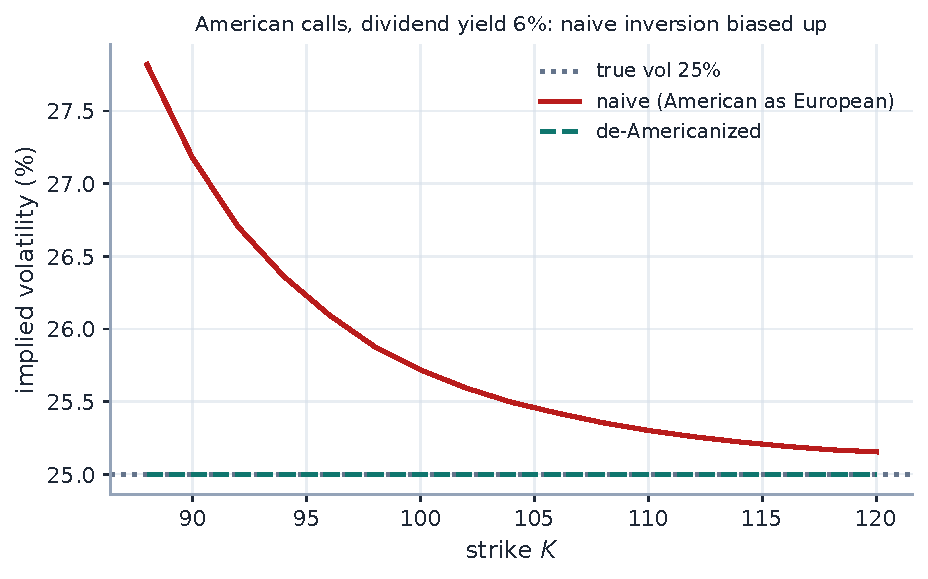
\includegraphics[width=\textwidth]{fig_deam_bias.pdf}\\[1pt]
{\footnotesize (a) naive vs de-Americanized implied vol}
\end{minipage}\hfill
\begin{minipage}{0.42\textwidth}\centering
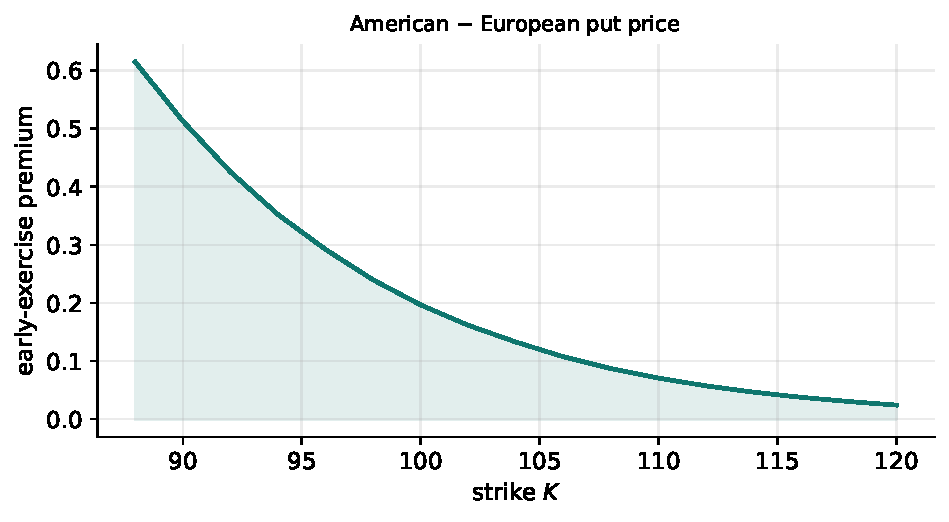
\includegraphics[width=\textwidth]{fig_deam_eep.pdf}\\[1pt]
{\footnotesize (b) the early-exercise premium (American $-$ European call)}
\end{minipage}
\caption{The naive European inversion of an American price is biased up by the
early-exercise premium; the de-Americanization returns the true volatility.
Synthetic American calls, $6\%$ dividend yield, true vol $25\%$.}
\label{fig:bias}
\end{figure}

%======================================================================
\section{Where the step sits: the production quote pipeline}
\label{sec:pipeline}

De-Americanization is one stage of quote preparation
(\texttt{volfit/api/quotes.py}). The full flow for one (ticker, expiry) is
\begin{center}
\ttfamily\small
raw chain $\to$ resolve $\fwd, D$ $\to$ OTM / tick screens $\to$ root on mid
$\to$ shift bid/mid/ask $\to$\\ normalized call $\to$ total variance $\to$
optional convex repair $\to$ model.
\end{center}
In words: the forward and discount are resolved first (put--call parity plus the
American de-bias of \cref{sec:carry}); the OTM side of the book is kept --- puts
for $K<\fwd$, calls for $K\ge\fwd$, because the OTM option carries the vega and
the tight relative spread --- and tick-noise / missing-side screens run; then, on
American chains only, each surviving \emph{mid} is de-Americanized.

\subsection{One root per strike, spread preserved}
\label{sec:eephat}

Given the American mid $A^{\mathrm{mid}}$ at a strike, the pipeline solves for
the volatility $\sigma^*$ at which the CRR American tree of \cref{sec:tree}
reprices it, then reprices the \emph{European} leg at that same volatility:
\begin{equation}
A_{\mathrm{CRR}}(\sigma^*)=A^{\mathrm{mid}},\qquad
E^{\mathrm{mid}}=P_{\Black}(\sigma^*),\qquad
\widehat{\mathrm{EEP}}=\max\!\big(A^{\mathrm{mid}}-E^{\mathrm{mid}},\,0\big).
\label{eq:eephat}
\end{equation}
The clamp at zero exists because the premium is theoretically nonnegative while
quote noise (and tree error) can dip the estimate below; it is one-sided by
design, and \cref{sec:convex} returns to its cost. The \emph{same}
$\widehat{\mathrm{EEP}}$ is subtracted from bid, mid and ask, so the quoted
dollar spread is preserved at the cost of one root find per strike instead of
three. Quotes the tree cannot invert keep $\widehat{\mathrm{EEP}}=0$ and their
raw prices fall through to the European static-bounds filter
(\cref{sec:numerics}).

\subsection{Into model space: parity, variance, clocks}

After the shift, the adjusted prices $p$ enter the ordinary European pipeline:
normalization to undiscounted forward units and put--call parity conversion of
the (OTM) puts to normalized calls,
\begin{equation}
c=\frac{p}{D\fwd}\ \ \text{(calls)},\qquad
c=\frac{p}{D\fwd}+1-e^{\logm}\ \ \text{(puts)},
\label{eq:parity}
\end{equation}
then a strike-by-strike inversion to total implied variance $\tvar$. Strikes
whose bid, mid or ask violates the static bounds $(1-e^{\logm})^+<c<1$ are
dropped (a one-sided band cannot be weighted), and a wing filter removes strikes
beyond $Z_{\max}=4$ ATM standard deviations.

One clock subtlety: the total variance $\tvar$ is inverted from the
\emph{price}, so it is clock-independent; only the \emph{reported} implied vol
depends on the working clock, $\text{iv}=\sqrt{\tvar/\tau}$. The
$\sigma^*$ of \cref{eq:eephat} is a calendar-time Black vol used transiently
inside the premium estimate; the vol a user sees on screen for the same quote can
differ because $\tau\ne t$ when event weighting is on (Note~00).

%======================================================================
\section{The pricing tree}
\label{sec:tree}

\subsection{Cox--Ross--Rubinstein}

The American value is computed by a Cox--Ross--Rubinstein binomial tree
\cite{CoxRossRubinstein1979}. With $N$ steps of size $\Delta t=t/N$, the spot
moves by $u=e^{\sigma\sqrt{\Delta t}}$ or $d=1/u$ each step, with risk-neutral
up-probability
\begin{equation}
p=\frac{e^{(r-q)\Delta t}-d}{u-d},\qquad 0<p<1,
\label{eq:crr_p}
\end{equation}
($r$ the rate, $q$ a continuous carry yield). The condition $0<p<1$ is the CRR
no-arbitrage requirement $d<e^{(r-q)\Delta t}<u$; it fails only for extreme
drift-to-vol ratios, and the scalar path then \emph{raises} rather than silently
mis-pricing (the batch path differs; \cref{sec:numerics}). The tree rolls back
from the payoff with discounting $e^{-r\Delta t}$, taking
$\max(\text{continuation},\text{intrinsic})$ at each node for the American
feature. The European value is the same recursion without the intrinsic
comparison. Stripped of the escrowed-dividend machinery, the kernel is a dozen
lines (this reproduces \texttt{binomial\_price} at $q=0$ to $10^{-10}$; the
European leg matches Black--Scholes to $2\times10^{-3}$ at depth):

\begin{lstlisting}[caption={The CRR backward induction with early exercise
(distilled from \texttt{core/american.py}).},label={lst:crr}]
def crr_price(is_call, s, k, t, sigma, r, n=501, american=True):
    dt = t/n; u = np.exp(sigma*np.sqrt(dt)); d = 1/u
    p = (np.exp(r*dt) - d)/(u - d); disc = np.exp(-r*dt)   # risk-neutral up-prob
    sT = s * u**np.arange(-n, n+1, 2)                      # terminal spots
    v = np.maximum(sT-k, 0.0) if is_call else np.maximum(k-sT, 0.0)
    for m in range(n-1, -1, -1):                          # roll back one layer
        v = disc*(p*v[1:] + (1-p)*v[:-1])                 # continuation value
        if american:                                     # early-exercise test:
            sM = s * u**np.arange(-m, m+1, 2)             #   max(continuation,
            v = np.maximum(v, sM-k if is_call else k-sM)  #       intrinsic)
    return v[0]
\end{lstlisting}

\subsection{Carry and dividends: what the tree actually uses}
\label{sec:carry}

For a real single name a flat continuous yield is a crude proxy: the call-side
early-exercise decision keys on discrete ex-dates. Production therefore chooses,
per (ticker, expiry), \emph{one} of two carry models for the tree
(\texttt{volfit/api/quotes.py}, \texttt{volfit/data/dividends.py}):

\begin{itemize}[leftmargin=1.6em]
\item \textbf{Discrete cash schedule, $q=0$.} When the dividend model supplies
cash dividends with ex-dates in $(0,t]$, the tree prices them by the
\emph{escrowed-spot} method \cite{Hull2018}: the present value of future
dividends is stripped from the spot to form the diffusing base lattice, and the
actual spot at each node is the base plus the PV of dividends not yet paid ---
recombining (cash drops otherwise break recombination) while exercising against
the true cum-dividend spot. The cash amounts are \emph{rescaled} by
\begin{equation}
\alpha=\frac{S-\fwd e^{-rt}}{\sum_i D_i e^{-r\tau_i}}
\label{eq:alpha}
\end{equation}
so the escrowed-tree forward $(S-\mathrm{PV}_0)e^{rt}$ reproduces the resolved
forward \emph{exactly}: the timing stays the forecast, the amounts bend to the
market. A non-physical $\alpha$ ($\le0$ or absurdly large) rejects the schedule.
\item \textbf{Continuous carry fallback.} Otherwise the tree runs on the
$(r,q)$ implied by the resolved pair $(\fwd,D)$: $r=-\log(D)/t$,
$q=r-\log(\fwd/S)/t$.
\end{itemize}

The two never coexist inside one tree: it is cash-with-$q{=}0$ or
continuous-yield, and \cref{eq:alpha} is what keeps the cash choice consistent
with a forward whose level partly reflects yield-like far-tail effects.

\begin{remark}[The apparent circularity, resolved]
De-Americanization needs $(\fwd,D)$; but put--call parity --- the source of
$(\fwd,D)$ --- is an \emph{equality only for European options}, so raw American
mids bias the parity regression. Production resolves this in order: the parity
regression runs first, then \texttt{\_refine\_american}
(\texttt{volfit/data/forwards.py}) de-biases it with a \emph{coarse} de-Am pass
--- including, where the de-Americanized put and call IVs fail to join at the
money, a rate bisection that zeroes that gap (the joint $(r,\fwd)$ refinement;
the ATM-kink case file of Note~06). Only then does the \emph{precise} per-quote
de-Americanization of this note run, under the refined carry. The refinement
uses fewer bisections and a coarser tolerance than quote prep --- it needs the
carry to a few bps, not the quote to sub-bp.
\end{remark}

%======================================================================
\section{The root find: control variate and error budget}
\label{sec:map}

\subsection{Tree inversion as a control variate}

De-Americanization is a one-dimensional root find. Given an American quote $A$
at $(S,K,t,r,q)$,
\begin{equation}
\boxed{\;\text{find }\sigma^*:\ \text{CRR}_{\text{Am}}(\sigma^*)=A,\quad
\text{return }\sigma^*\text{ as the European-equivalent Black vol.}\;}
\label{eq:deam}
\end{equation}
This is the standard desk workflow --- convert American quotes to
pseudo-European quotes, then calibrate a European model --- studied critically
by Burkovska et al.~\cite{Burkovska2018}: pragmatic and fast, not theoretically
exact outside the model.

\begin{heuristic}
Why is the \emph{tree's} $\sigma^*$ the right European volatility? Because the
tree is a \emph{control variate} for the early-exercise feature. The market
price differs from the European price we want by an EEP we cannot observe; the
tree supplies a model EEP as a function of $\sigma$. Subtracting it at
$\sigma^*$,
\begin{equation}
A_{\mathrm{mkt}}
-\underbrace{\big[A_{\mathrm{CRR}}(\sigma^*)-E_{\mathrm{CRR}}(\sigma^*)\big]}_{\text{model EEP at }\sigma^*}
= E_{\mathrm{CRR}}(\sigma^*)\;\approx\;P_{\Black}(\sigma^*),
\label{eq:cv}
\end{equation}
where the first equality uses the defining property
$A_{\mathrm{CRR}}(\sigma^*)=A_{\mathrm{mkt}}$ and the last step is tree
discretization only ($\sim10^{-5}$ of spot at the scalar depth). So $\sigma^*$
is the de-Americanized Black vol: the early-exercise premium cancels in the
control variate, and the tree's \emph{level} error largely cancels with it ---
the tree only has to price the American/European \emph{difference} well. The
method is exact in the model and robust in practice because the EEP is a smooth,
slowly varying function of $\sigma$.
\end{heuristic}

\subsection{Static bounds, bracketing, and failure semantics}
\label{sec:numerics}

A price below intrinsic (impossible for an American option) or above the static
upper bound ($S$ for a call, $K$ for a put) yields \texttt{nan}, mirroring the
fitter's convention for unusable quotes. The bracket lower end is lifted just
above the CRR drift floor $\sigma\sqrt{\Delta t}>|r-q|\Delta t$ so
\cref{eq:crr_p} stays valid, and the upper end is expanded until the price is
bracketed, capped at $\sigma=\text{\texttt{SIGMA\_HI}}=4$.

The scalar and batch paths deliberately differ in how they fail. The
\emph{scalar} path (one quote, Brent root find, $N=501$) \emph{raises} on an
invalid CRR probability --- a single mis-priced input should be loud. The
\emph{batch} path must survive mixed inputs, so invalid lanes (static-bound
violations, a deep-ITM put priced at its early-exercise floor below the
drift-floor model price, never-bracketed quotes) return \texttt{NaN} and the
rest of the chain proceeds. Upstream, quote prep treats a \texttt{NaN} root as
``no premium estimate'': $\widehat{\mathrm{EEP}}=0$, and the untouched band is
left for the European static-bound filters to keep or drop.

\subsection{Depth, bisection, and the error budget}

Two depths are used. The scalar path uses $N=\text{\texttt{DEFAULT\_STEPS}}=501$;
the batch path a coarser $N=\deamsteps$ tree and a fixed \deambisect-sweep
bracketed bisection. The bisection count was tuned down from $45$ to
\deambisect\ at no measurable accuracy cost ($<0.01$ vol bp drift, test-locked),
a $\sim1.8\times$ saving on the isolated de-Am rail.

Separating the error sources of the returned $\sigma^*$:
\begin{itemize}[leftmargin=1.6em,itemsep=1pt]
\item \textbf{Root tolerance.} \deambisect\ halvings of a $\le4.0$ bracket leave
$\sim2.4\times10^{-7}$ of $\sigma$ ($\sim0.002$ vol bp) --- pure bisection
uncertainty, negligible.
\item \textbf{Finite tree.} The $\deamsteps$-step European leg prices within a
few $10^{-4}$ of Black; through vega that is a few vol bps on liquid quotes ---
visible as the $\pm2$ vol bp residuals on the real-chain OTM calls of
\cref{sec:real} (where the true EEP is $\approx0$ and the tree error is all
that remains). The scalar 501-step leg is $\sim10\times$ tighter.
\item \textbf{Carry / dividend model.} A wrong forward, discount or cash
schedule biases $\sigma^*$ directly; de-Americanization inherits, and cannot
repair, the inputs of \cref{sec:carry} (see the closing caution of
\cref{sec:real}).
\item \textbf{Market vs model.} The CRR diffusion between ex-dates and the
one-sided clamp of \cref{eq:eephat} are modelling choices; their footprint is
the wing non-convexity that \cref{sec:convex} repairs.
\end{itemize}

\begin{caution}
The tree depth is a numerical-target knob, not a free speed dial. Cutting the
batch depth from $\deamsteps$ to $128$ is faster (the backward induction is
$O(N^2)$, so $\sim2\times$) but shifts the priced European leg by $\sim15$ vol
bps --- i.e.\ it changes the \emph{answer}, not just the runtime. The depth is
held at $\deamsteps$ and speed is bought elsewhere (the Numba kernel,
\cref{sec:numba}).
\end{caution}

%======================================================================
\section{A worked example, by the numbers}
\label{sec:example}

\begin{example}[title={Case file: one strike of \cref{fig:bias}}]
Setup: American call, $S=100$, $K=\deamwexstrike$, $t=0.5$, $r=2\%$, $q=6\%$,
true volatility $\sigma=25\%$, scalar tree depth $N=501$. The production tree
prices
\[
A_{\mathrm{CRR}}=\deamwexam,\qquad
E_{\mathrm{CRR}}=\deamwexeu,\qquad
\widehat{\mathrm{EEP}}=A_{\mathrm{CRR}}-E_{\mathrm{CRR}}=\deamwexeep .
\]
With a $6\%$ yield against a $2\%$ rate, exercising early to capture the
dividend stream is valuable on an ITM call --- about $4.4\%$ of this option's
value. Handing the American price to the analytic European Black inversion
(production's normalization: $c=A/(D\fwd)$ at $\logm=\log(K/\fwd)$) returns
\[
\sigma_{\text{naive}}=\deamwexnaive\%,
\]
a $+\deamwexbias$ vol bp phantom: the inversion attributes the premium to
volatility. Solving \cref{eq:deam} instead gives
$\sigma^*=\deamwexdeam\%$ --- the truth, to bisection tolerance. Every number
above is generated by \texttt{figures/gen\_deam.py} from
\texttt{core/american.py}; the full-strike sweep is \cref{fig:bias}.
\end{example}

%======================================================================
\section{Caching and the compiled kernel}
\label{sec:cache}

\subsection{The prepared-quote cache key}

De-Americanized, inverted quotes depend only on the \emph{data} entering quote
preparation --- never on any fit setting. The pipeline memoizes each node's
prepared quotes on a content-digest key (\texttt{volfit/api/service.py}) built
from:
\begin{center}
\ttfamily\small
(ticker, expiry, data\_version, forward, discount, cash-dividend digest,
$t$, $\tau$, as-of)
\end{center}
\texttt{data\_version} is the raw chain's identity (bumped on fetch or chain
invalidation); the forward/discount absorb the forward policy and manual edits;
the cash digest absorbs the dividend model and rate; calendar $t$ drives the
CRR carry and discounting; $\tau$ is included because the \emph{cached reported
IV band} is quoted in the event-weighted clock ($\text{iv}=\sqrt{\tvar/\tau}$),
so an event edit must re-key. A change to any of these re-runs the trees;
model choice, penalties, quote weights and optimizer tuning do \emph{not} ---
so the de-Am cost is paid once per genuine data change and is then free across
an entire calibration sweep. A conservative pre-screen (non-positive bids, a
buffered wing cut) additionally drops quotes that cannot survive the static
bounds \emph{before} any tree runs, and is output-preserving by construction.

\subsection{The Numba kernel}
\label{sec:numba}

The hot path de-Americanizes a whole chain. The NumPy batch vectorizes across
quotes but allocates $(n_{\text{quotes}},m)$ slabs per time step; the compiled
kernel does a single scalar CRR per quote with no per-step allocation ---
precomputed power tables, the escrow lattice constants hoisted out, and a
\texttt{prange} parallel loop over quotes.

\begin{perfbox}
On a \deamchainn-quote synthetic chain the kernel runs in \deamnumbams\,ms
versus \deamnumpyms\,ms for the NumPy fallback --- \deamspeedup$\times$.
The comparison is like-for-like: \emph{both} timings call the public
\texttt{deamericanize\_batch} dispatch (identical static screens, identical
drift-floor bracket), the NumPy leg by forcing the fallback; both paths run
once untimed first (JIT compile excluded) and the fastest of five repeats is
reported; the generator \emph{raises} unless the two paths return identical
finite/\texttt{NaN} lanes (\deamchainfinite\ of \deamchainn\ here --- the rest
are deep-ITM puts at their exercise floor, correctly \texttt{NaN} on both) and
identical roots (observed max $|\Delta\sigma|=0$). Measured on a
\deamthreads-thread desktop; this uniform synthetic chain parallelizes
especially well --- the documented figure on wide \emph{real} chains is
$\sim60\times$. If Numba is unavailable the fallback serves with identical
results; the kernel agrees with the scalar tree to tree rounding.
\end{perfbox}

%======================================================================
\section{Cross-strike convexity: repairing the de-Americanized wings}
\label{sec:convex}

De-Americanization inverts each strike \emph{independently} --- its own root
find \eqref{eq:deam}, its own one-sided clamp \eqref{eq:eephat} --- with no
coupling across strikes. That independence is what makes the kernel
embarrassingly parallel (\cref{sec:numba}), but the European-equivalent call
prices $\{c(K_i)\}$ it hands the parity conversion \eqref{eq:parity} need not
come out \emph{convex} in the strike. To be precise about the mechanism:
independent inversion does not by itself create arbitrage --- if the input
prices were exactly consistent with one arbitrage-free model, the outputs would
be too. The non-convexity is injected by quote noise in sparse wings, the
one-sided $\max(\mathrm{EEP},0)$ clamp (a strike-local, asymmetric
perturbation), finite-tree error, and carry/model mismatch --- and per-strike
inversion simply has no cross-strike coupling with which to absorb any of it.

Convexity is not optional. Writing the undiscounted call as
$C(K)=\E^{\Q}[(S_T-K)^+]$, its second derivative in strike is the risk-neutral
density, $\partial^2C/\partial K^2=f_{S_T}(K)\ge0$: \emph{convexity of the call
curve in strike is exactly the no-butterfly-arbitrage condition}. On a discrete
strike grid the test is the divided second difference
\begin{equation}
\Delta^2_i=\frac{C_{i-1}(K_{i+1}-K_i)-C_i(K_{i+1}-K_{i-1})+C_{i+1}(K_i-K_{i-1})}
{K_{i+1}-K_{i-1}}\ \ge\ 0,
\label{eq:bfly_strike}
\end{equation}
non-negative iff $C$ is convex at $K_i$. Because the injected noise concentrates
in the sparse, low-vega wings, $\Delta^2_i$ can come out slightly negative there
--- a genuine (small) butterfly arbitrage in the \emph{input} handed to every
downstream model, and the seed of the put-wing violation of the Multi-Core
Sigmoid model that Note~03 dissects.

\begin{caution}
\textbf{The reverted global fix.} The first repair projected the \emph{whole}
call curve onto the convex cone with a free \emph{global} affine part. Repairing
a wing dip that way re-tilted the baseline and moved the at-the-money prices ---
prices the repair had no business touching. The ATM core is where vega peaks, so
the sub-penny price moves were \emph{small} in implied vol; but the core is also
where quotes are densest, spreads tightest, and fit weight heaviest, so the
unnecessary coherent shift --- and the discontinuity it opened against
neighbouring untouched quotes --- surfaced immediately as a visible ATM smile
gap on live SPY and NVDA. It was reverted. The lesson is about \emph{locality},
not vega: a repair aimed at the wings must be structurally incapable of moving
the trusted core, hence invariant~4.
\end{caution}

The shipped repair (\texttt{volfit/calib/convex\_deam.py}) is therefore
\emph{wing-only and band-constrained}, and honestly: \emph{approximate}. It acts
on the normalized OTM call curve \emph{after} the parity conversion
\eqref{eq:parity}. Strikes in the core $|z|\le Z_{\text{core}}=1$ are held
byte-identical. Each wing, anchored at its core boundary, is replaced by an
approximation to the $\ell^2$-closest curve that is simultaneously \emph{convex}
and \emph{inside the quoted band} --- the projection onto the intersection
$\mathcal C\cap\mathcal B$ of
\begin{equation}
\mathcal C=\{\hat C:\hat C\ \text{convex, leaving the anchor no flatter than the
core}\},\quad
\mathcal B=\{\hat C:C^{\text{bid}}\le\hat C\le C^{\text{ask}}\},
\label{eq:convex_sets}
\end{equation}
computed by \emph{at most 25 iterations} of Dykstra's alternating projection ---
the convex-cone step a non-negative-hinge least squares, the band step a clip.
The implementation does not certify that $\mathcal C\cap\mathcal B$ is nonempty
(a wing whose convexification demands leaving the band has no exact solution;
the iterate then lands near the band), does not post-check global convexity of
the final assembled curve, and by construction cannot repair a violation
\emph{inside} the held-fixed core. A common per-strike shift is applied to bid,
mid and ask so the \emph{spread is preserved}, and the repaired band is
re-inverted to total variance.

\begin{heuristic}
Why the band constraint is load-bearing. Plain convex projection of an illiquid,
genuinely non-convex wing is free to push a price all the way to the static
no-arb boundary --- and a wing call price at that boundary inverts to an absurd
implied volatility (a put wing was seen to jump from $27\%$ to $104\%$, itself
violating Lee's moment bound $\tvar(\logm)\le2|\logm|$ for large $|\logm|$;
Note~03), detonating the downstream fit. Confining the repaired price to the
\emph{quoted spread} bounds the correction to the market's own stated
uncertainty: the repair can move a price only as far as the bid--ask allows,
which is exactly as far as the quote is genuinely ambiguous.
\end{heuristic}

The repair is gated American-only and short-circuits on any curve already convex
to a tolerance $\text{CONVEX\_TOL}=10^{-3}$ (normalized price units), calibrated
so that dense liquid chains --- whose de-Am wings carry only $\sim\!10^{-4}$
rounding curvature --- are \emph{never} touched (byte-identical, ATM implied-vol
difference $\sim10^{-15}$), while genuinely arbitraged illiquid wings ($10^{-3}$
to $10^{-2}$) are repaired. On those illiquid nodes an ablation found the repair
both \emph{reduces} the fitted arbitrage and \emph{lowers} the in-sample error
--- the model no longer chases the arbitraged quotes --- and it composes with
the put-wing penalty of Note~03 (a Durrleman-style $g\ge0$ constraint on the
\emph{output} smile) rather than duplicating it: the de-Am repair removes the
arbitrage at the \emph{source}, and running both attains the penalty's
arbitrage removal at a fraction of its standalone in-sample cost.

%======================================================================
\section{Real-chain evidence, honestly labelled}
\label{sec:real}

The synthetic example of \cref{sec:example} controls the truth;
\cref{fig:deam_real,fig:deam_real_sel} show the effect on live market prices,
with nothing simulated --- and on two deliberately different populations.

\paragraph{The stress exhibit (\cref{fig:deam_real}).}
Every two-sided put quote of one captured SPY expiry (the Massive true-weekly
fixture \texttt{lv\_weekly\_massive.json}, as-of 2026-06-25; the December-2026
expiry, strikes $55\%$--$138\%$ of spot) is inverted both ways: naively through
the analytic European Black formula (production's inversion, what a fitter that
ignored early exercise would compute) and through the American tree
\eqref{eq:deam}. Since the EEP itself has \emph{price} units, what the wedge
between the curves shows is the \emph{model-implied IV effect} of the premium,
not an observed premium. Out of the money the two agree to a few vol bps; in
the money the wedge runs to a median \deamrealmedianitm\ vol bps across the
\deamrealnitm\ ITM puts, up to \deamrealmaxbias.

But this population is \textbf{not what Vol-Fitter fits}. Production keeps the
OTM side only --- puts below $\fwd$, calls above (\cref{sec:pipeline}) --- so
the ITM puts carrying the headline wedge are, in all but the thin band between
spot and the forward, exactly the quotes production \emph{discards} in favour
of their OTM call twins. \Cref{fig:deam_real} is an
economic stress illustration of what skipping de-Americanization would do to
the discarded side, not a statement of fit exposure.

\begin{figure}[H]
\centering
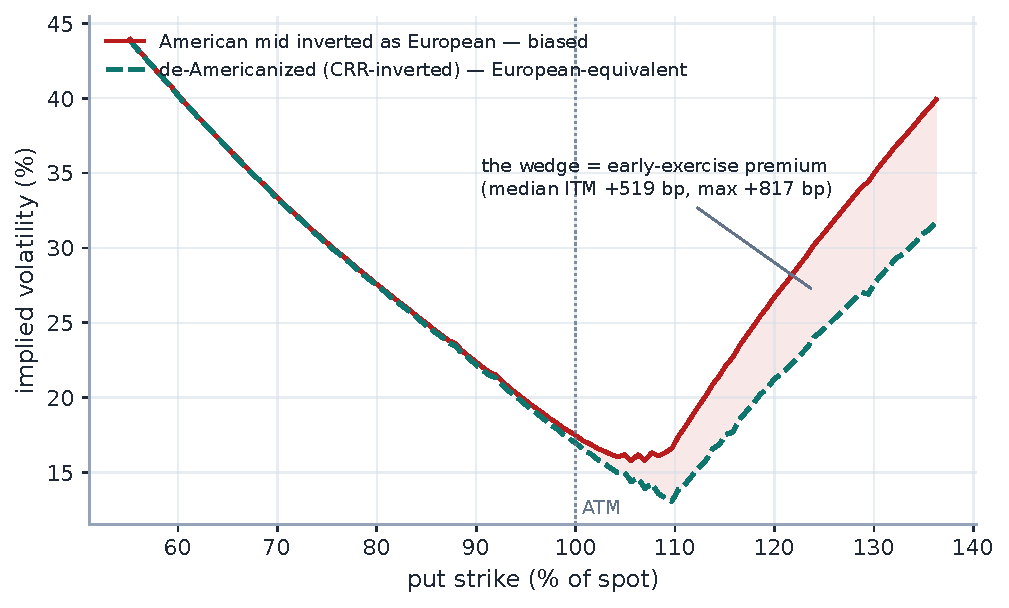
\includegraphics[width=0.82\textwidth]{fig_deam_real.pdf}
\caption{Real market data, one live SPY expiry (Massive capture, as-of
2026-06-25, December-2026): every two-sided put mid inverted as if European
versus de-Americanized. The ITM wedge --- median \deamrealmedianitm\ vol bps,
up to \deamrealmaxbias\ --- is the model-implied IV effect of the
early-exercise premium on a side production almost entirely \emph{discards}
for OTM calls: a stress exhibit, not the fitted population (that is
\cref{fig:deam_real_sel}). Carry supplied ($r=4.3\%$, $q=1.2\%$) because the
delayed capture's parity carry is unusable (Note~06). Generated by
\texttt{figures/gen\_deam\_real.py} from the production CRR machinery.}
\label{fig:deam_real}
\end{figure}

\paragraph{The fitted population (\cref{fig:deam_real_sel}).}
Running the same two-way inversion on the quotes production actually selects ---
\deamrealseln\ OTM puts and calls of the same expiry, after the tick-noise
floor and the $Z_{\max}$ wing filter of \cref{sec:pipeline} --- the de-Americanization
moves the implied vol by a median $|\cdot|$ of \deamrealselabsmedian\ vol bps,
maximum \deamrealselmax\ (selected OTM puts: median
$\deamrealselputmedian$\,bp, max $\deamrealselputmax$; selected OTM calls:
median $\deamrealselcallmedian$\,bp, max $\deamrealselcallmax$). This is the
honest statement of what de-Americanization is worth on this liquid,
moderate-carry ETF chain at six months: a few vol bps in the body, tens in the
put wing --- material against the fitter's sub-vol-bp error budgets, an order
of magnitude below the stress exhibit. (The small \emph{negative} values on the
calls are the $\deamsteps$-step tree's discretization against analytic Black
--- the finite-tree line of the error budget --- not a negative premium.)
Single names with hard dividends and higher rates sit between the two panels.

\begin{figure}[H]
\centering
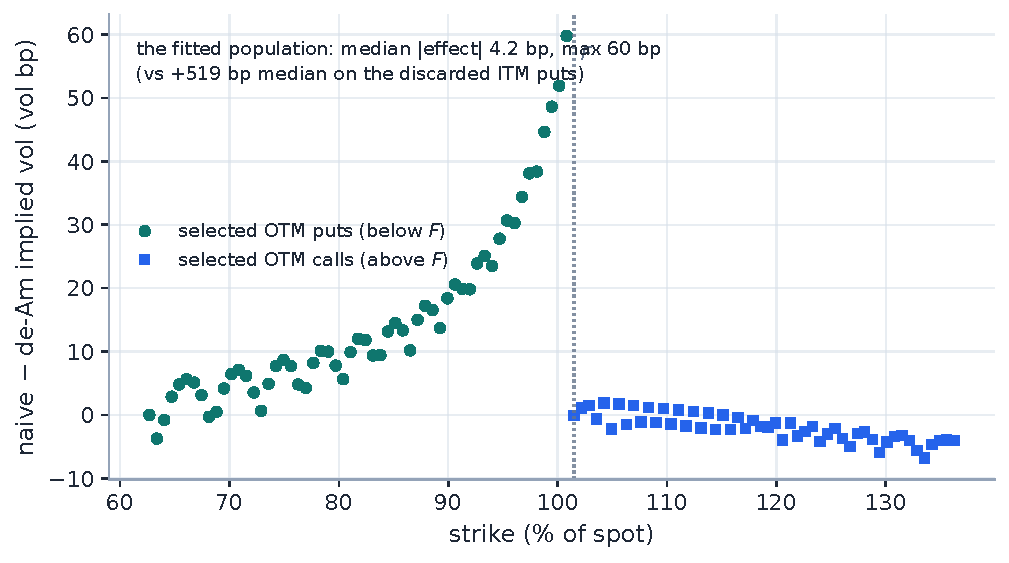
\includegraphics[width=0.82\textwidth]{fig_deam_real_selected.pdf}
\caption{The same expiry, restricted to the quotes production actually fits
(OTM puts below $\fwd$, OTM calls above): the de-Am IV effect is a median
$|\cdot|$ of \deamrealselabsmedian\ vol bps, max \deamrealselmax\ in the put
wing --- the fit's real de-Am exposure, an order of magnitude below the
discarded-ITM stress exhibit. Generated by
\texttt{figures/gen\_deam\_real.py}.}
\label{fig:deam_real_sel}
\end{figure}

One honesty note on inputs: the delayed-tier capture's parity-implied carry is
unphysical (Note~06 documents how such feeds synthesize chains from
per-contract IVs at $\fwd=S$, $D=1$, destroying parity information), so the
carry here is supplied explicitly --- $r=4.3\%$ money-market, $q=1.2\%$ SPY
dividend yield (mid-2026) --- a live instance of the caution below.

\begin{caution}
What the model does and does not cover. The tree supports a deterministic
scheduled cash-dividend path (escrowed, forward-consistent via
\cref{eq:alpha}) \emph{or} an equivalent continuous-carry fallback, with a CRR
diffusion between ex-dates. It does not model stochastic jumps, uncertain
dividend timing or amounts, stochastic rates, or stochastic borrow. And
$\sigma^*$ is only as good as the resolved forward and dividend inputs
(Note~06): the method removes the \emph{early-exercise} bias; it cannot repair
a wrong forward.
\end{caution}

%======================================================================
\section{What is original, and future directions}
\label{sec:original}

The control-variate view of tree inversion is folklore; the contributions here
are the \emph{allocation-free Numba kernel} (the per-step allocation, not the
arithmetic, was the NumPy bottleneck), the \emph{prepared-quote content cache}
that scopes de-Am cost to genuine data changes rather than to fit iterations,
the \emph{measured} depth/bisection tuning that cut work without moving the
numerical target, and the \emph{wing-only, band-constrained convexity repair}
(\cref{sec:convex}) that removes the butterfly arbitrage the per-strike
inversion leaves in the sparse wings while holding the dense ATM core exactly
fixed. The natural next step --- documented but not yet shipped --- is to seed
the bracket with a fast analytic American approximation (Barone-Adesi--Whaley
\cite{BaroneAdesiWhaley1987} or Bjerksund--Stensland
\cite{BjerksundStensland2002}) so each tree starts near its root, composing
with the kernel for a further constant-factor win; these are \emph{seeds}, not
the answer, so they change no contract.

\appendix
%======================================================================
\section{Hyperparameter atlas}
\label{app:atlas}

\begin{longtable}{p{0.26\textwidth}p{0.14\textwidth}p{0.52\textwidth}}
\caption{De-Americanization hyperparameters (all hidden / internal).}\label{tab:atlas}\\
\toprule Constant & Default & Role\\ \midrule
\endfirsthead \toprule Constant & Default & Role\\ \midrule \endhead
\texttt{DEFAULT\_STEPS} & $501$ & Scalar CRR tree depth; European leg matches Black to $\sim10^{-5}$.\\
\texttt{DEFAULT\_BATCH\_STEPS} & $\deamsteps$ & Batch/kernel tree depth.\\
\texttt{BATCH\_BISECTIONS} & $\deambisect$ & Bracketed-bisection sweeps ($\sim0.002$ vol bp).\\
\texttt{SIGMA\_LO} & $10^{-4}$ & Lower vol bracket floor; production lifts it
above the CRR drift floor, $\max(10^{-4},\,1.5\,|r-q|\sqrt{t/N})$.\\
\texttt{SIGMA\_HI} & $4.0$ & Upper vol bracket cap.\\
escrow PV & --- & Discrete-cash-dividend escrowed-spot lattice
(forward-consistent rescale \cref{eq:alpha}, cap $\alpha\le5$).\\
pre-screen buffer & $1.5\times$ & Wing buffer for the conservative bid/bounds pre-screen.\\
prepared-quote key & --- & Cache key (ticker, expiry, raw-chain
\texttt{data\_version}, forward, discount, dividends, $t$, $\tau$, as-of).\\
\texttt{convex\_deam} & \texttt{true} & Enable the wing-only convex de-Am repair
(\cref{sec:convex}); American chains only, European a no-op.\\
$Z_{\text{core}}$ & $1.0$ & ATM core half-width (units of $\sqrt{\tvar_{\atm}}$) held
byte-identical by the repair.\\
\texttt{CONVEX\_TOL} & $10^{-3}$ & Convexity short-circuit: a curve convex to this
(normalized price) is left untouched.\\
Dykstra iterations & $25$ & Cap on the alternating projection of
\cref{sec:convex} (approximate, not certified).\\
\bottomrule
\end{longtable}

%======================================================================
\section{Performance notes}
\label{app:perf}

\begin{enumerate}[leftmargin=1.6em]
\item \textbf{Numba kernel} (\cref{sec:numba}). Single scalar CRR per quote, no
per-step allocation, precomputed powers, \texttt{prange} over quotes; measured
\deamspeedup$\times$ over the NumPy fallback on a \deamchainn-quote synthetic
chain (\cref{tab:deam_time}; $\sim60\times$ documented on wide real chains).
Both paths through the public dispatch; identical roots asserted before the
number is reported. Graceful NumPy fallback.
\item \textbf{Bisection tuning.} $45\to\deambisect$ sweeps, $<0.01$ vol bp drift,
$\sim1.8\times$ on the isolated rail.
\item \textbf{Prepared-quote content cache.} De-Am re-runs only on a genuine
data change, never on fit-setting changes --- free across a calibration sweep.
\item \textbf{Output-preserving pre-screen.} Drops unusable quotes before the tree,
by construction not changing any surviving result.
\item \textbf{Future (not shipped):} BAW / BS-2002 analytic bracket seeds to start
each tree near its root.
\end{enumerate}

\begin{table}[H]
\centering
\caption{De-Americanizing a \deamchainn-quote synthetic chain
(\deamchainfinite\ invertible on both paths, identical roots;
$\deamsteps$-step trees, \deambisect\ bisections; one untimed warm-up per path,
fastest of five repeats, \deamthreads\ threads).}
\label{tab:deam_time}
\begin{tabular}{lrr}
\toprule
Path & time (ms) & relative\\
\midrule
NumPy fallback (same dispatch) & \deamnumpyms & $1\times$\\
Numba kernel & \deamnumbams & \deamspeedup$\times$\\
\bottomrule
\end{tabular}
\end{table}

%======================================================================
\section{Reference implementation: convexity building blocks}
\label{app:ref}

The convexity test \eqref{eq:bfly_strike} and the convex-cone half of the wing
repair are compact; the listing below shows these two \emph{building blocks},
not the shipped repair. \texttt{min\_butterfly} is the divided second
difference (its minimum is $\ge0$ iff the curve is convex, i.e.\
butterfly-free); \texttt{convex\_fit} is the convex-cone projection --- the
$\ell^2$-closest convex curve leaving the core anchor, written as an affine
part plus non-negative hinge knots, so $\delta_j\ge0$ is exactly the convexity
constraint. The production module (\texttt{calib/convex\_deam.py}) composes
\texttt{convex\_fit} with a bid/ask clip inside the capped Dykstra alternation
of \cref{sec:convex} and additionally handles duplicate strikes (multiple
listings at one strike) and the core/wing gating --- none of which is shown
here. Both listings reproduce their production counterparts to $10^{-9}$.

\begin{lstlisting}[caption={The no-butterfly test and the convex wing fit (distilled
from \texttt{calib/convex\_deam.py}).}]
def min_butterfly(K, C):                     # >= 0  <=>  C convex in strike (no bfly)
    a, b = K[1:-1]-K[:-2], K[2:]-K[1:-1]     # left / right strike gaps
    fly = C[:-2]*b - C[1:-1]*(a+b) + C[2:]*a # divided second difference
    return (fly / (a+b)).min()

def convex_fit(u, c, slope_floor):           # L2-closest convex curve, anchor c[0]
    cols = [u] + [np.maximum(u-u[j], 0.0) for j in range(1, len(u)-1)]
    A = np.column_stack(cols)                # [u, (u-u_j)_+ ...] : affine + hinges
    lb = np.zeros(A.shape[1]); lb[0] = slope_floor   # leaving slope >= core; delta_j >= 0
    x = lsq_linear(A, c - c[0], bounds=(lb, np.inf)).x
    return c[0] + A @ x                       # convex by construction (delta_j >= 0)
\end{lstlisting}

%======================================================================
\section{Traceability}
\label{app:trace}

\begin{longtable}{p{0.34\textwidth}p{0.12\textwidth}p{0.24\textwidth}p{0.22\textwidth}}
\caption{Claim $\to$ equation $\to$ code $\to$ test.}\label{tab:trace}\\
\toprule Claim & Equation & Module & Test\\ \midrule
\endfirsthead \toprule Claim & Equation & Module & Test\\ \midrule \endhead
$\sigma^*$ root = de-Americanized Black vol; static-bound / drift-floor
\texttt{NaN} semantics & \eqref{eq:deam}, \eqref{eq:cv} &
\texttt{volfit/core/american.py} & \texttt{tests/test\_american.py}\\
Spread-preserving $\widehat{\mathrm{EEP}}$ shift of bid/mid/ask; OTM selection;
parity conversion & \eqref{eq:eephat}, \eqref{eq:parity} &
\texttt{volfit/api/quotes.py} & \texttt{tests/test\_quotes\_deam.py}\\
$24$-bisection drift $<0.01$ vol bp vs the 45-sweep baseline & --- &
\texttt{volfit/core/american.py} & \texttt{tests/test\_quotes\_deam.py}\\
Escrowed cash schedule, forward-consistent rescale & \eqref{eq:alpha} &
\texttt{volfit/data/dividends.py} & \texttt{tests/test\_discrete\_deam.py}\\
Kernel $=$ NumPy fallback to tree rounding (incl.\ cash dividends) & --- &
\texttt{volfit/core/american\_numba.py} & \texttt{tests/test\_american\_numba.py}\\
Prepared-quote cache: invalidation table & --- &
\texttt{volfit/api/service.py} & \texttt{tests/test\_prepared\_cache\_key.py}\\
Wing repair: ATM core byte-identical, band-stay, convexity gate &
\eqref{eq:bfly_strike}, \eqref{eq:convex_sets} &
\texttt{volfit/calib/convex\_deam.py} & \texttt{tests/test\_convex\_deam.py}\\
Joint $(r,\fwd)$ American de-bias joins the ATM sides & --- &
\texttt{volfit/data/forwards.py} & \texttt{tests/test\_forward\_debias.py}\\
\bottomrule
\end{longtable}

\begin{thebibliography}{9}
\bibitem{CoxRossRubinstein1979} J.~Cox, S.~Ross and M.~Rubinstein. Option pricing:
a simplified approach. \emph{J.\ Financial Economics}, 7(3):229--263, 1979.
\bibitem{Hull2018} J.~Hull. \emph{Options, Futures, and Other Derivatives}.
Pearson, 10th edition, 2018. (Escrowed-dividend binomial trees.)
\bibitem{BaroneAdesiWhaley1987} G.~Barone-Adesi and R.~Whaley. Efficient analytic
approximation of American option values. \emph{J.\ Finance}, 42(2):301--320, 1987.
\bibitem{BjerksundStensland2002} P.~Bjerksund and G.~Stensland. Closed form
valuation of American options. Working paper, NHH, 2002.
\bibitem{Burkovska2018} O.~Burkovska et al. Calibration to American options:
numerical investigation of the de-Americanization method.
\emph{arXiv:1611.06181}.
\end{thebibliography}

\end{document}
